We can write equation \eqref{4/7/Eq a} as,
\begin{align} \label{4/7/Eq b}
9 x^2 + 4 y^2 - 36 = 0
\end{align}
which has parameters
\begin{align}
\vec{V}=\myvec{9 & 0 \\ 0 & 4} , \vec{u}=\myvec{0 \\ 0} , f = -36
\end{align}
The vertex of ellipse is obtained as 
\begin{align} \label{4/7/Eq d}
\vec{c} &= - \vec{V}^-^1 \vec{u}
% \end{align}
% We know,
% \begin{align}
% \vec{V}^-^1 = \frac{1}{\begin{vmatrix}\vec{V}\end{vmatrix}} Adj \vec{V}
% \end{align}
% Substituting the values of \begin{vmatrix}\vec{V}\end{vmatrix} and Adj \vec{V} we get,
% \begin{align}
% \vec{V}^-^1 = \frac{1}{36} \myvec{4 & 0 \\ 0 & 9}^\top   
%  = \myvec{\dfrac{4}{36} & 0 \\ 0 & \dfrac{9}{36}} 
% \end{align}
% Substituting values in equation \eqref{4/7/Eq d} we get the vertex of the ellipse,
% \begin{align}
&=\myvec{0 \\ 0}
\end{align}
The length of semi major axis and semi minor axis are given by,
\begin{align} \label{4/7/Eq e}
\sqrt{\frac{\vec{u}^\top \vec{V}^-^1 \vec{u} - f}{ \lambda_1}} = 3   ,   \sqrt{\frac{\vec{u}^\top \vec{V}^-^1 \vec{u} - f}{ \lambda_2}} = 2
%  \end{align}
% Solving equation \eqref{4/7/Eq e} we get,
% \begin{align} 
\implies \lambda_1 = 4   ,   \lambda_2 = 9
\end{align}
The eccentricity of ellipse is given by,
\begin{align} \label{4/7/Eq f}
e &= \sqrt{1 - \frac{\lambda_1}{\lambda_2}}
% \end{align}
% Substituting the values in equation \eqref{4/7/Eq f} we get,
% \begin{align}
 &= \frac{\sqrt{5}}{3}
\end{align}
The constant parameter for the directrices of ellipse  is  given by,
\begin{align} \label{4/7/Eq g}
c = \frac{e \vec{u}^\top \vec{n} \pm \sqrt{e^2 (\vec{u}^\top n)^2 - \lambda_2 (e^2 - 1) (\norm{\vec{u}}^2 - \lambda_2 f)}}{\lambda_2 e (e^2 - 1)}
\end{align}
Where
\begin{align}
\vec{n} = \sqrt{\lambda_2} \textbf p_1 = \myvec{0 \\ 1}
\end{align}
As
\begin{align}
 \vec{p_1} = \frac{1}{\sqrt{9}} \myvec{0 \\ 1}
\end{align}
Substituting the values in equation \eqref{4/7/Eq g} we get directrices of the ellipse,
\begin{align}
c = \pm \frac{9}{\sqrt{5}}
\end{align}
The foci of ellipse are given by,
\begin{align} \label{4/7/Eq h}
\vec{F} = \frac{c e^2 \vec{n} - \vec{u}}{\lambda_2}
\end{align}
Substituting the respective values in equation \eqref{4/7/Eq h} we get,
\begin{align}
\vec{F}=\myvec{0 \\ \dfrac{\sqrt{5}}{3}}
\end{align}
\centering
\begin{figure}[!ht]
\centering
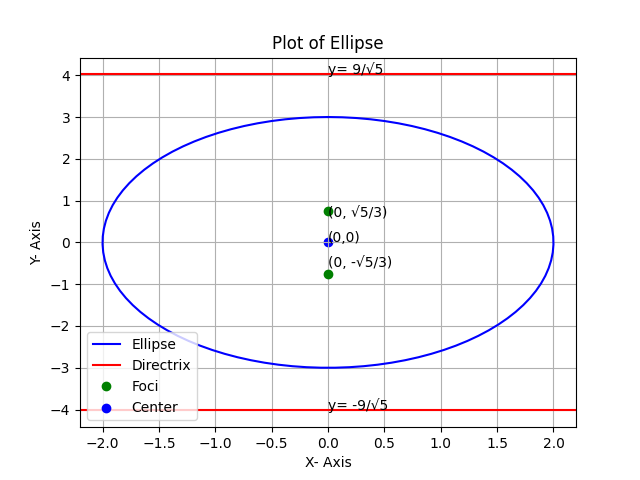
\includegraphics[width=\columnwidth]{solutions/4/7/Figure_1.png}
\caption{Plot of the Ellipse with vertex \vec{c}}
\label{4/7/fig}
\end{figure}